\documentclass[11pt,a4paper]{article}
\usepackage[margin=0.85in]{geometry}
\usepackage[T1]{fontenc}
\usepackage{lmodern}
\usepackage{amsmath,amssymb,mathtools}
\usepackage{graphicx,booktabs,array,enumitem}
\usepackage[dvipsnames]{xcolor}
\usepackage{microtype}
\usepackage{caption}
\usepackage{listings}
\usepackage{hyperref}
\hypersetup{colorlinks=true,linkcolor=MidnightBlue,urlcolor=MidnightBlue,
  pdfauthor={},pdfsubject={Reinforcement learning worked solutions}}
\setlength{\parindent}{0pt}
\setlength{\parskip}{6pt}
\setlist{nosep,leftmargin=*}
\setlength{\emergencystretch}{2em}
\captionsetup{font=small,labelfont=bf}
\lstset{basicstyle=\ttfamily\small,breaklines=true,
  columns=fullflexible,keepspaces=true,showstringspaces=false,
  commentstyle=\color{gray},keywordstyle=\color{MidnightBlue},
  aboveskip=6pt,belowskip=6pt}
\newcommand{\E}{\mathbb{E}}
\newcommand{\R}{\mathbb{R}}
\newcommand{\norm}[1]{\left\lVert #1\right\rVert}
\newcommand{\sg}{\operatorname{stopgrad}}
\DeclareMathOperator*{\argmax}{arg\,max}
\DeclareMathOperator*{\argmin}{arg\,min}
\newcommand{\studytitle}[1]{%
  \hypersetup{pdftitle={#1 - Worked Solutions}}%
  {\small\color{MidnightBlue} BASICRL\quad /\quad WORKED SOLUTIONS}\par
  \vspace{5pt}{\LARGE\bfseries #1}\par\vspace{5pt}}
\newcommand{\historical}{\textbf{Experiment status.} The following numbers and
  curves are retained from earlier runs, not from a rerun of the revised
  reference code. They are examples for interpretation, not performance guarantees.\par}

\begin{document}
\studytitle{Model-Based Reinforcement Learning}

\section{Expert policy and transition data}
Train a PPO expert in the wrapped reaching environment, then collect
$\mathcal D_E=\{(s_t,a_t,s_{t+1})\}$ by executing that expert. Each tuple must
contain the pre-action observation, the executed action, and its resulting
next observation. Do not replace a terminal next observation with the next
episode's reset observation.

The exercise uses a fixed target and a progress reward
\[
 r_t=10(d_t-d_{t+1}),\qquad d_t=\norm{g-x_t}_2,
\]
with success termination and a 50-step limit. An undiscounted episode return
telescopes to $10(d_0-d_T)$. It depends on initial and final distances as well
as success; success rate is therefore a complementary metric, not an
equivalent representation of return.

Use separate environment instances for data collection, policy training,
and evaluation. Vectorized environments must also contain independent
simulator instances, rather than several wrappers around one shared simulator.

\section{Learning the world model}
Fit a deterministic model $f_\psi(s,a)$ to predict $s'$. The reference uses
an MLP with two ReLU hidden layers:
\[
 f_\psi(s,a)=W_3\,\operatorname{ReLU}
    \big(W_2\,\operatorname{ReLU}(W_1[s;a]+b_1)+b_2\big)+b_3.
\]
Concatenating along the last axis maps a batch $(B,d_s)$ and $(B,d_a)$
to $(B,d_s+d_a)$. Train on an 80\% split and evaluate on the remaining
20\%, with the loss
\[
 L_{\rm model}=\frac{1}{N d_s}\sum_{i=1}^N
                      \norm{f_\psi(s_i,a_i)-s'_i}_2^2.
\]
The retained setup uses 50 epochs, Adam, and learning rate $10^{-4}$.
Its double-precision model requires both state and action inputs to match
the parameter dtype. Evaluation uses \texttt{eval()} and disables gradients.
Average batch losses using sample counts so a small final batch is not
given the same weight as a full batch.

A transition-level split is a convenient learning exercise but can place
nearby, strongly correlated transitions on both sides. For a stronger
generalization assessment, split by complete trajectories and keep an
independent real-environment policy evaluation set.

\newpage
\section{Training a policy inside the learned model}
Replace the transition dynamics with $s_{t+1}=f_\psi(s_t,a_t)$, retain the
target, and compute reward and success from the simulated gripper position.
For the flattened observation convention here, goal coordinates occupy
indices 0--2 and gripper coordinates indices 3--5. Freeze the learned dynamics
while PPO learns its policy. Use the same 50-step limit in model and real
evaluation, and propagate reset seeds through the environment.

Model quality must be judged under the states and actions visited by the
\emph{learner}, which can differ from the expert's data. Under additional
assumptions of a one-step prediction error $\delta$ and a Lipschitz constant
$L$ for the true closed-loop transition map, an illustrative recursion is
\[
 e_{t+1}\leq Le_t+\delta,\qquad
 e_t\leq\delta\sum_{k=0}^{t-1}L^k\quad(e_0=0).
\]
These extra assumptions are not established by a small validation MSE. The
recursion explains how one-step error can accumulate; it is not a fitted
performance bound for this experiment. The policy can also exploit errors
in learned dynamics, producing high model return but weaker real return.

\section{Aggregating learner data}
Execute the first learned policy in the real environment to obtain
$\mathcal D_L$, then fit a fresh model on
$\mathcal D_{\rm agg}=\mathcal D_E\cup\mathcal D_L$. Keep aligned triples
when shuffling. Train another PPO policy in this second model and evaluate
it in both environments using the same protocol.

This resembles DAgger in expanding coverage toward learner-visited states.
The supervision is different: here the environment supplies next states;
DAgger queries an expert for action labels. Aggregation can improve coverage
but does not guarantee improvement for every dataset or optimization run.

\section{Retained numerical results}
\historical
\begin{center}
\begin{tabular}{lrrr}
\toprule Policy training environment & Model return & Real return & Real success\\\midrule
Real environment (expert) & -- & 1.5267 & 78\%\\
Expert-data world model & 1.6798 & 1.2117 & 67\%\\
Aggregated-data world model & 1.6611 & 1.5738 & 88\%\\\bottomrule
\end{tabular}
\end{center}
The recorded model-validation MSE is approximately $2\times10^{-6}$ for
the first model. The aggregated model was printed as \texttt{0.000000};
six-decimal rounding does not establish exact zero error.

\newpage
\section{Reading the results correctly}
The first model-trained learner loses about $0.4681$ return when moving from
the learned environment to the real one. After aggregation, the analogous
gap is about $0.0873$. This is consistent with better coverage and reduced
model exploitation, although the records do not isolate either mechanism.

The aggregated learner's recorded real return $1.5738$ exceeds the expert's
$1.5267$, and its recorded success rate $88\%$ exceeds $78\%$. Thus these
numbers do \emph{not} support a statement that it still underperforms the
expert. The honest conclusion is that it performs better in these saved
evaluations. Repeated seeds, matched initial states, and uncertainty estimates
would be needed to argue a reliable advantage.

\begin{figure}[h!]
\centering
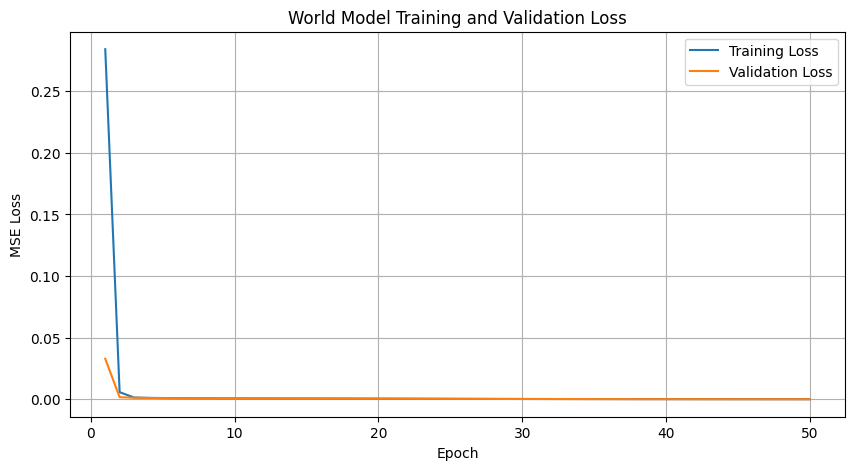
\includegraphics[width=0.47\linewidth]{figures/world-model-loss.png}\hfill
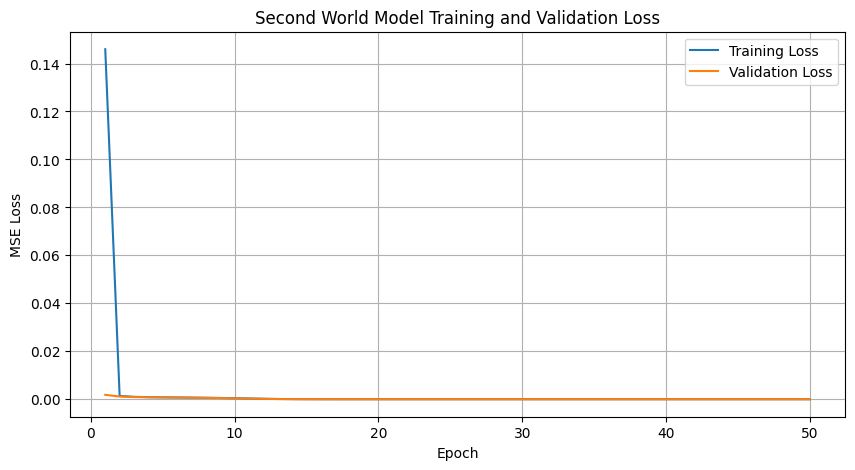
\includegraphics[width=0.47\linewidth]{figures/aggregated-model-loss.png}
\caption{Retained training and validation losses for the first and aggregated
world models. Small one-step MSE does not certify long-horizon policy fidelity.}
\end{figure}
\begin{figure}[h!]
\centering
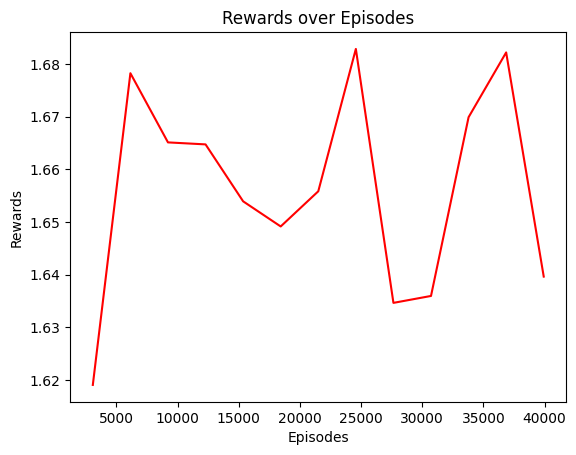
\includegraphics[width=0.47\linewidth]{figures/model-policy-return.png}\hfill
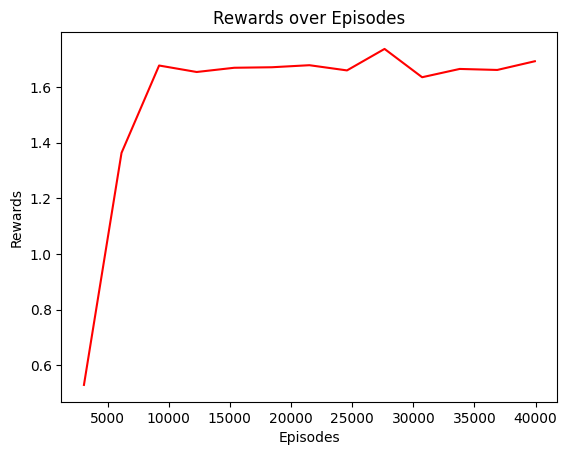
\includegraphics[width=0.47\linewidth]{figures/aggregated-policy-return.png}
\caption{Retained callback evaluation curves. Their original horizontal label
says ``Episodes''; the callback actually records training timesteps.}
\end{figure}

\textbf{Solution scope.} The model objective and data-aggregation procedure
specify the implementation. Numerical observations are historical and
unreplicated. The revised environment uses independent simulator instances,
consistent horizons, and explicit dtype handling; these revisions require
new experiments before performance claims can be attached to the current code.
\end{document}
